\subsection*{Optimisation/Runtime Efficiency}
As code is generated considerations of efficiency can be made such that the object code becomes more efficient than other alternatives.
Such optimisations consists of considerations like memory allocation, pipelining, parallelisation and other considerations that may have an impact on execution time.
To do an efficient and complete analysis of how to optimise code, information of the situation in program is required.
This is where \gls{gamble} is at a disadvantage due to the fact that \gls{gamble} distances its programmers from controlling where the code is performed and instead does so seamlessly.
Information about how e.g. a for-loop could be transformed into a kernel does not exist in \gls{gamble} which makes it difficult to do this.
The seamless use of the \acrshort{gpu} means that information is lackluster and therefore all computations may not be fully optimised in terms of where to execute, this is one of the tradeoffs \gls{gamble} makes.
If \gls{gamble} were to require more information, the simplicity and seamless use of the \acrshort{gpu} would be lost.

As previously mentioned due the object code being OpenCL C certain considerations pertaining to instruction handling and register allocation etc. are not of interest for optimisation for this compiler.
Instead the optimisation here resides in when to use the \acrshort{gpu}, optimising the generated C code as well as the OpenCL kernels.

As \gls{gamble} is attempting to seamlessly use the \acrshort{gpu} to increase performance, knowing when the use of the \acrshort{gpu} will actually be a benefit is an important point in the code generation process.
As mentioned to do this effectively, the compiler would require more information about the computations which are to be done than can be read from the syntax of \gls{gamble}.
Therefore the project group have decided that it is better to be sure that a computation can benefit from the \acrshort{gpu}, rather than risking moving computations that wont benefit as well as those that will.
As such only those operations that the project group knows have a possibility of benefiting from the parallel abilities of the \acrshort{gpu} will be executed on the \acrshort{gpu}.

%Knowing when to use GPU
Even though a computation can be parallelised, does not necessarily mean it should as is evident in \myref{image:benchmark}.
This is an opportune point for optimising the object code to use the \acrshort{gpu} only when it leads to an increase in execution speed.
A possibility of doing so would be to analyse whether or not an operation is both big enough and compatible with the \acrshort{gpu}.
Performing such an analysis increases the time it takes to do code generation.
Because of the difficulty to discern not only if there will be an actual increase, but also if any custom functions created by the programmer are fit to run on the \acrshort{gpu} this optimisation is not made.
Instead only vector and matrix operations already defined in the language will be performed on the \acrshort{gpu}.

%Optimising C code(CPU)

%Optimising OpenCL Kernals
A function that is to be run on the \acrshort{gpu} is in the OpenCL framework called a kernel.
Since kernel code uses explicit memory handling, one must choose what memory space to allocate ones variables in.
In the different kernels the better one utilises its memory the faster a kernel can be executed, as a result of the memory used being located higher in the memory hierarchy.
\begin{figure}[h!]
\centering
 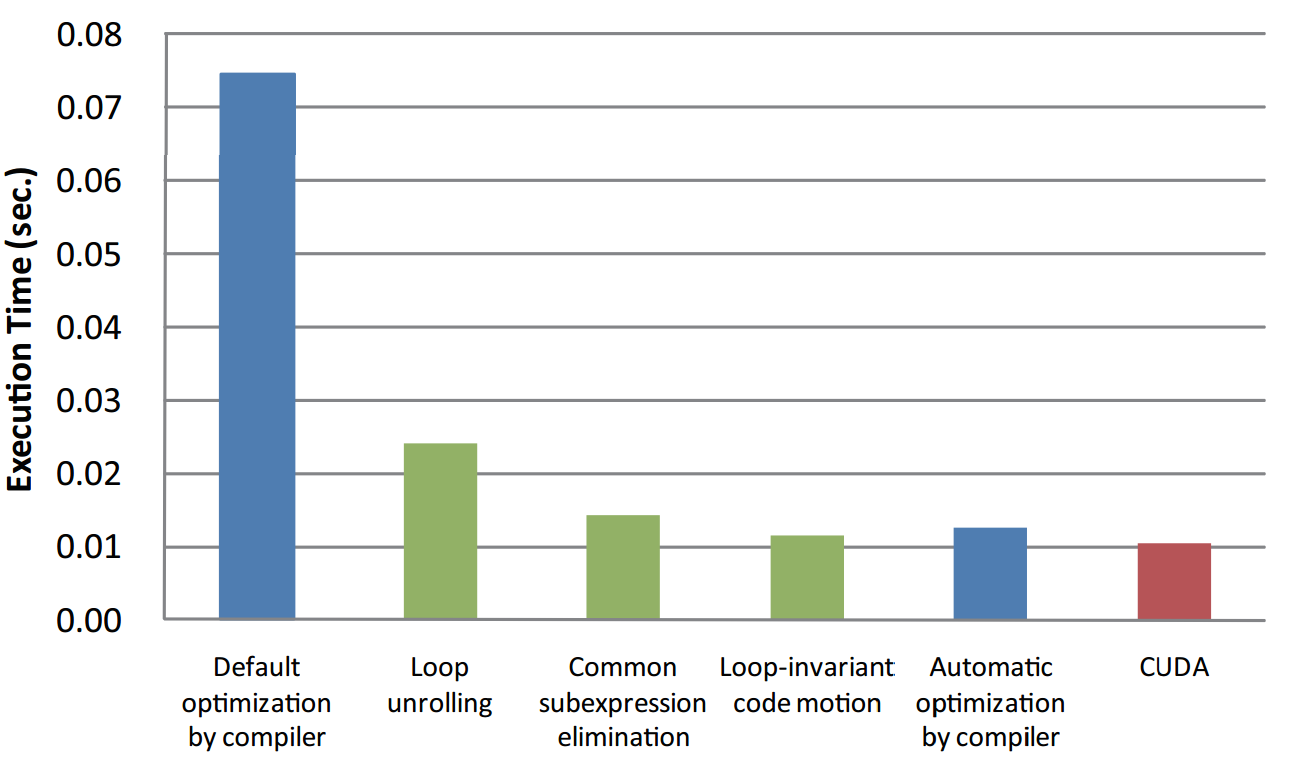
\includegraphics[width=1\textwidth]{figures/opencloptimisation.png} % trim=4.85cm 15cm 0.85cm 1cm
\caption{Execution speed of a matrix multiplication with different optimisation levels. \citep{CUDAOpenCLOptimisation}}\label{image:OpenCLOptCompare}
\vspace{-15pt}
\end{figure}
As seen on \myref{image:OpenCLOptCompare} some possible optimisations include loop unrolling, common sub-expression elimination and loop-invariant code motion. 
These are taken as specific examples in this comparison because these optimisations are made in the \acrlong{ptx} code that CUDA compiles.
An OpenCL C compiler also provides the option of doing optimisation upon the code, however it would seem that depending on the \acrshort{gpu} and platform one is working on optimisations must be altered.
Furthermore the ideal work-group size changes, making universal optimisation a difficult task to take on.
OpenCL uses JIT compilation to generate binary code to the appropriate device it is working with.
While this allows it to be used on more platforms than one like CUDA, it also results in compiler optimisations being quite time-consuming and thus increases the total execution time.\citep{CUDAOpenCLOptimisation}